
\begin{figure}[h!]
\textbf{Tema d'Esame di Gennaio 2017}\\ \\
Un disco metallico viene lanciato con velocità $v$ nel punto A del tratto AB, di lunghezza
$l = 4 m$, in modo che percorra tale tratto e poi il tratto BC, di lunghezza uguale al precedente
e inclinato di un angolo $\alpha$ = 60$^{\circ}$ rispetto all’orizzontale. Il tratto AB è senza attrito, mentre tra il disco e il tratto BC vi è attrito ($\mu$D = $0.6$). Quanto vale $v$ se il disco arriva in C con velocità nulla? 
\\
	\begin{center}
		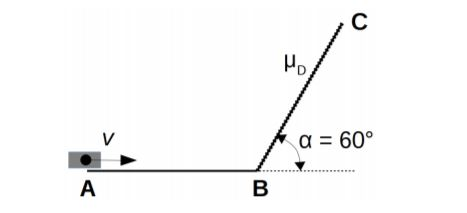
\includegraphics[scale=0.5]{ES2/GEN022017.jpg}
	\end{center}
\end{figure}


\begin{figure}[h!]
\textbf{Tema d'Esame di Febbraio 2017}\\ \\
Nel sistema in figura la molla ha una costante elastica di $1.20 N/cm$. Il piano sul quale si
muove la pallina è inclinato di 10.0$^{\circ}$ rispetto all’orizzontale. La molla viene inizialmente compressa di $5.00 cm$. Si calcoli la velocità che raggiunge una pallina di massa $100 g$ quando la molla viene rilasciata. Si trascuri ogni attrito e la massa della molla.
\\
	\begin{center}
		
\includegraphics[scale=0.5]{ES2/FEB022017.jpg}
	\end{center}
\end{figure}


\begin{figure}[h!]
\textbf{Tema d'Esame di Giugno 2017}\\ \\
Un blocco metallico di massa $m = 0.5 kg$, partendo da fermo, viene lasciato
scivolare lungo un piano inclinato con un angolo $\alpha$ = 30$^{\circ}$ rispetto all’orizzontale e con un coefficiente di attrito dinamico $\mu$D = $0.25$. Dopo aver percorso il tratto AB del piano inclinato lungo $85 cm$, il blocco raggiunge una superficie orizzontale, priva di attrito, sulla quale è posta una molla ($k = 35 N/m$). Il blocco urta la molla e la comprime. Qual’è la compressione massima della molla?
\\
	\begin{center}
		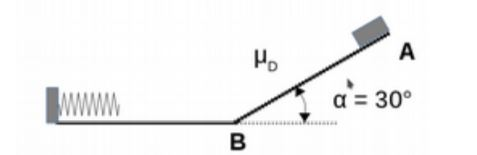
\includegraphics[scale=0.5]{ES2/GIU022017.jpg}
	\end{center}
\end{figure}

\begin{figure}[h!]
\textbf{Tema d'Esame di Luglio 2017}\\ \\
Una molla con costante elastica $77.61 N/cm$, viene compressa prima di lanciare una palla verso un piano inclinato. La palla ha massa $1 kg$ e il piano inclinato è alto $H = 4.36 m$. Quanto deve essere compressa la molla affinché la palla arrivi con una velocità di $15 m/s$ in cima al piano?
\\
	\begin{center}
		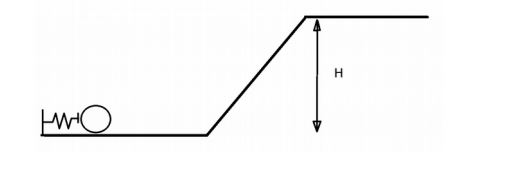
\includegraphics[scale=0.6]{ES2/LUG022017.jpg}
	\end{center}
\end{figure}


\begin{figure}[h!]
\textbf{Tema d'Esame di Settembre 2017}\\ \\
Una pallina abbandona un piano inclinato ($\theta$ = 30$^{\circ}$) da un’altezza pari a $5 m$ e tocca il suolo dopo $0,8 s$. Si determini il modulo della velocità con cui abbandona il piano inclinato. 
\\
	\begin{center}
		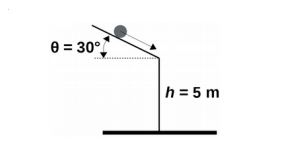
\includegraphics[scale=1]{ES2/SET022017.jpg}
	\end{center}
\end{figure}